% !TeX root = srs.tex
% !TeX program = pdflatex
\documentclass[11pt,a4paper]{article}

% Allow inclusion of PDF figures exported with newer PDF versions
\pdfminorversion=7

% =====================
% Packages
% =====================
\usepackage[top=0.9in,left=0.9in,right=0.9in,bottom=1.2in]{geometry}
\usepackage{array}
\usepackage{ragged2e}
\usepackage{setspace}
\usepackage{hyperref}
\usepackage{enumitem}
\usepackage{graphicx}
\usepackage{eso-pic}  % Background images
\usepackage{fancyhdr}
\usepackage{tabularx}
\usepackage{booktabs}
\usepackage{multirow}
\usepackage{float}
\usepackage{xcolor}
\usepackage{parskip}
\usepackage{amsmath}
\usepackage{amssymb}
\usepackage{colortbl}
\usepackage{longtable}
\usepackage{textcomp}
\usepackage{caption}
\usepackage{bookmark}
\hypersetup{hidelinks}
\definecolor{tableheader}{RGB}{240, 240, 240}
\definecolor{tablerow}{RGB}{250, 250, 250}
\frenchspacing

% =====================
% Font (pdflatex-friendly Arial-like)
% =====================
\usepackage[T1]{fontenc}
\usepackage[scaled=0.95]{helvet}
\renewcommand{\familydefault}{\sfdefault}

\setstretch{1.0}

% =====================
% BACKGROUND IMAGES SETUP
% =====================
% Cover page (Page 1): Brigman_Letterhead.pdf
% All other pages: Brigman_Paper.pdf
\AddToShipoutPictureBG*{%
  \AtPageLowerLeft{%
    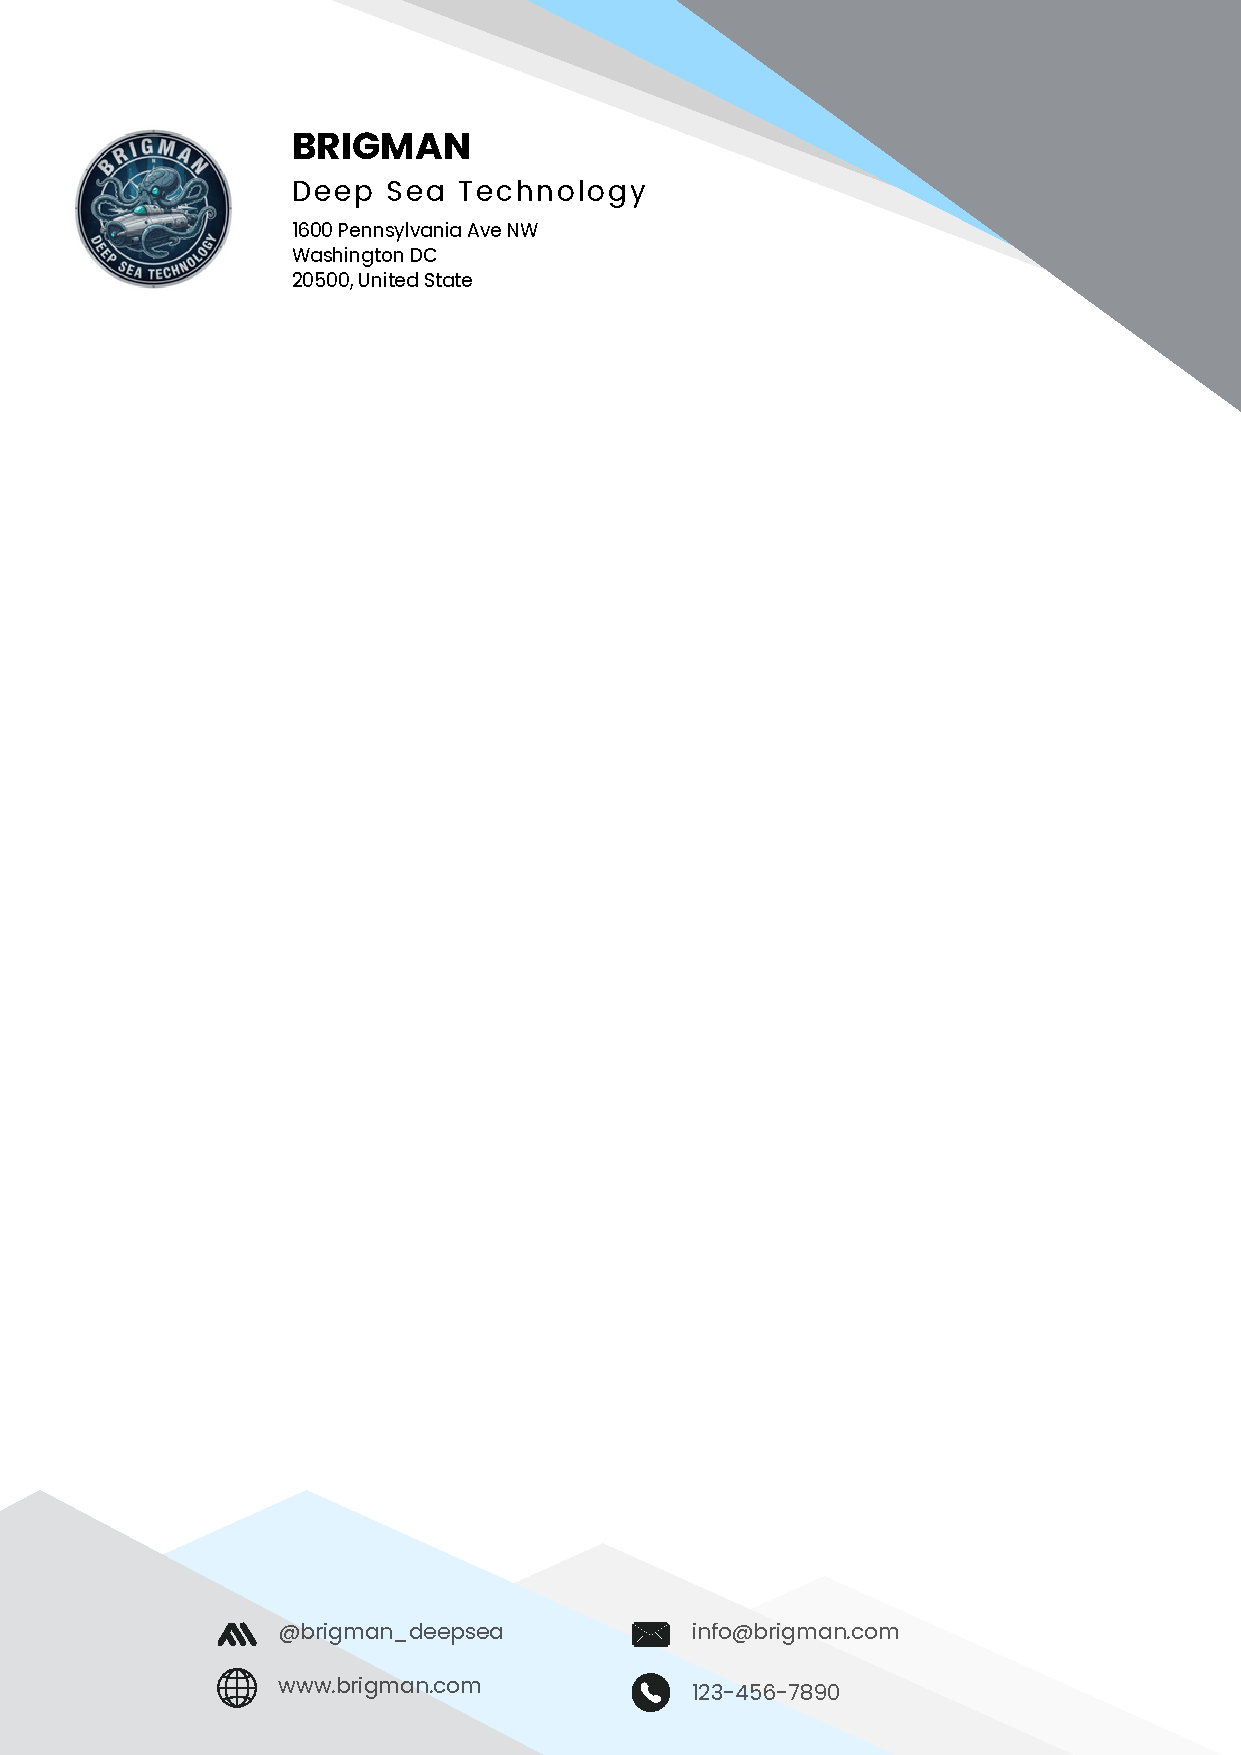
\includegraphics[width=\paperwidth,height=\paperheight]{../templates/Brigman_Letterhead.pdf}%
  }%
}
\AddToShipoutPictureBG{%
  \ifnum\value{page}>1
    \AtPageLowerLeft{%
      
\includegraphics[width=\paperwidth,height=\paperheight]{../templates/Brigman_Paper.pdf}%
    }%
  \fi
}

% =====================
% Header/Footer (page numbers must appear)
% =====================
\pagestyle{fancy}
\fancyhf{}
\lhead{\textbf{Brigman Deep Sea Technology}}
\rhead{Software Requirements Specification (SRS)}
\cfoot{\thepage}
\renewcommand{\headrulewidth}{0.4pt}
\setlength{\headheight}{20pt}

\begin{document}

% =====================
% COVER PAGE (no page number)
% =====================
\thispagestyle{empty}
\fancyhf{}
\lhead{}
\rhead{}
\cfoot{}
\renewcommand{\headrulewidth}{0pt}

\newgeometry{top=5.2cm,left=0.9in,right=0.9in,bottom=1.2in}

\begin{center}

\includegraphics[width=0.4\textwidth]{../templates/brigman logo.png}\\[0.5cm]

\LARGE\textbf{Software Requirements Specification (SRS)}\\[0.4cm]
\large\textbf{Abyss Navigator Suite Project}\\[0.6cm]

\textbf{\Large Brigman Deep Sea Technology}\\
\today
\end{center}

\begin{table}[H]
\centering
\small
\renewcommand{\arraystretch}{2.0}
\begin{tabular}{|>{\raggedright\arraybackslash}m{0.25\textwidth}|>{\raggedright\arraybackslash}m{0.2\textwidth}|>{\raggedright\arraybackslash}m{0.25\textwidth}|>{\raggedright\arraybackslash}m{0.2\textwidth}|}
\hline
\rowcolor{tableheader}
\textbf{Brigman Team Member} & \textbf{Department} & \textbf{Role} & \textbf{Employee ID} \\
\hline
Muhammad Ridwan Putra Jasni & Requirements Engineering & Lead Business Analyst & BDST-RE-BA-001 \\
\hline
Chng Zong Han & Requirements Engineering & Business Analyst & BDST-RE-BA-002 \\
\hline
Lin Yuhao & Requirements Engineering & Business Analyst & BDST-RE-BA-003 \\
\hline
Muhammad Mikhail Bin Mazlan & Requirements Engineering & Business Analyst & BDST-RE-BA-004 \\
\hline
Kannan s/o Rajamohan & Requirements Engineering & Business Analyst & BDST-RE-BA-005 \\
\hline
\end{tabular}
\end{table}

\restoregeometry
\newpage

% Restore standard headers for rest of document
\pagestyle{fancy}
\fancyhf{}
\lhead{\textbf{Brigman Deep Sea Technology}}
\rhead{Software Requirements Specification (SRS)}
\cfoot{\thepage}
\renewcommand{\headrulewidth}{0.4pt}
\setlength{\headheight}{20pt}

% =====================
% FRONT MATTER
% =====================
\renewcommand{\contentsname}{Table of Contents}
\thispagestyle{empty}
\tableofcontents
\newpage

\section*{Revision History}
\addcontentsline{toc}{section}{Revision History}

\begin{table}[H]
\centering
\small
\renewcommand{\arraystretch}{1.2}
\begin{tabular}{|c|c|>{\raggedright\arraybackslash}p{0.22\textwidth}|>{\raggedright\arraybackslash}p{0.45\textwidth}|}
\hline
\rowcolor{tableheader}
\textbf{Version} & \textbf{Date} & \textbf{Author} & \textbf{Reason for Changes} \\
\hline
0.1 & \today & BDST Requirements Team & Initial SRS draft structured using the Karl E. Wiegers SRS template (1999) and IEEE 830-aligned categorization. \\
\hline
\end{tabular}
\end{table}

\newpage

% =====================
% 1. INTRODUCTION
% =====================
\section{Introduction}

\subsection{Purpose}
This Software Requirements Specification (SRS) defines the software requirements for the \textbf{Abyss Navigator Suite}, an unmanned deep-sea submersible fleet control system for Triton Deepwater. It is intended to be the baseline agreement for design, implementation, verification, and change control.

\subsection{Document Conventions}
\textbf{Template source.} This SRS is structured using the \textit{Software Requirements Specification} template by \textbf{Karl E. Wiegers (1999)} (provided in \texttt{References/srs\_template-ieee.pdf}), adapted to incorporate the course rubric requirements (requirements tree, codification, iRTM, and change mitigation).

\textbf{Normative language.} All requirements use \textbf{shall} to indicate mandatory behavior.

\textbf{Codification (mandatory).} The following ID schemes are used throughout:
\begin{itemize}[leftmargin=*,nosep]
  \item \textbf{Software requirements:} \texttt{<DOMAIN>-<FEATURE>-<NNN>} (e.g., \texttt{SAF-EMG-001}).
  \item \textbf{Technology requirements:} \texttt{TECH-<AREA>-<NNN>} (e.g., \texttt{TECH-PLAT-001}).
  \item \textbf{Quality model features:} \texttt{QUAL-<AREA>-<NNN>} (e.g., \texttt{QUAL-SAF-001}).
  \item \textbf{iRTM entries:} \texttt{RTM-<NNN>} (e.g., \texttt{RTM-001}).
  \item \textbf{Change mitigation controls:} \texttt{CHG-<AREA>-<NNN>} (e.g., \texttt{CHG-CTRL-001}).
\end{itemize}

\textbf{Priority levels.} Priority is recorded as \textbf{Essential}, \textbf{Desirable}, or \textbf{Acceptable} to align with the Project Specification.

\subsection{Intended Audience and Reading Suggestions}
This SRS is intended for Triton Deepwater stakeholders, the Brigman development and verification teams, project management, and independent auditors. Readers should begin with Sections 1--3 (scope, constraints, requirements tree and codification) before using Section 4 (requirements) and Sections 7--8 (traceability and change mitigation).

\subsection{Product Scope}
The Abyss Navigator Suite enables unmanned missions executed autonomously, remotely supervised from a surface or mothership environment, with controlled intervention, safe emergency handling, and operational traceability.

\subsection{References}
\begin{itemize}[leftmargin=*,nosep]
  \item Triton Deepwater, \textit{Project Specification: The Abyss Navigator Suite}, ICT2113, 2026.
  \item Brigman Deep Sea Technology, \textit{Software Requirements Analysis Report (BCIC Methodology)}, 2026.
  \item Kevin Anthony Jones, \textit{Labtorial Guide for Class Project: Reqrs now \& near future}, Dec 2025.
  \item Kevin Anthony Jones, \textit{Guide Rubric for Assessment of Deliverables}, Jan 2026.
  \item Karl E. Wiegers, \textit{Software Requirements Specification Template}, 1999.
\end{itemize}

% =====================
% 2. OVERALL DESCRIPTION
% =====================
\section{Overall Description}

\subsection{Product Perspective}
The Abyss Navigator Suite is a new software product that coordinates multiple unmanned submersibles and interfaces with Triton-provided mission sensors, communications links, and external reporting/analysis environments.

\begin{figure}[H]
\centering
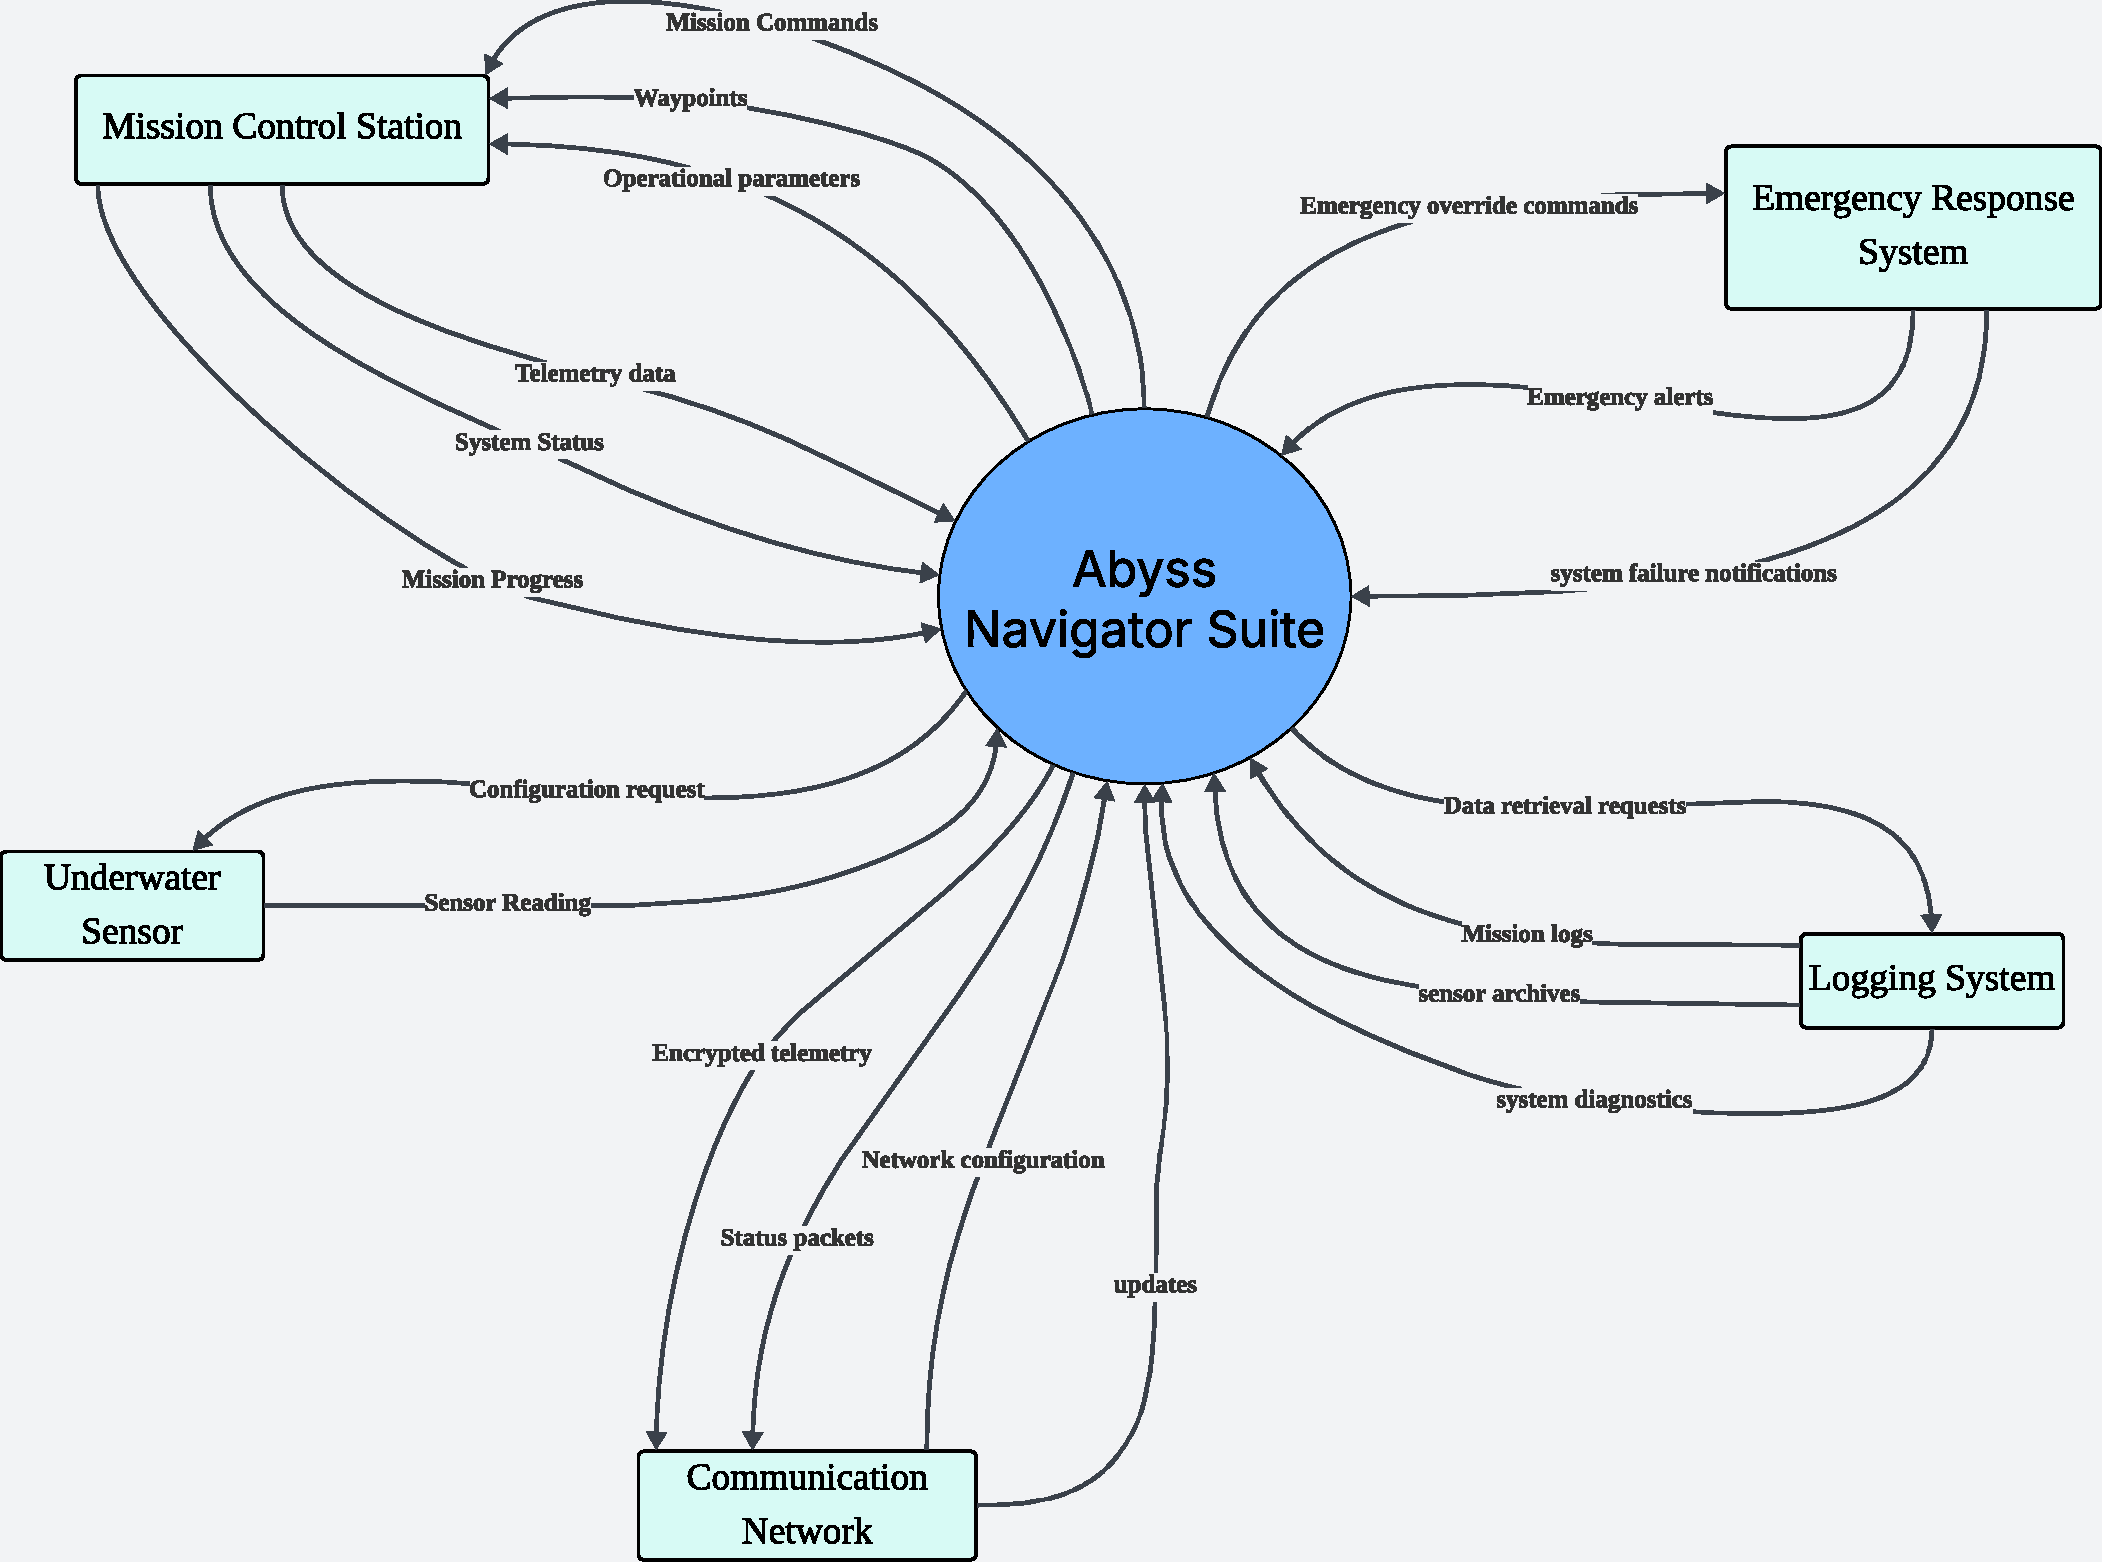
\includegraphics[width=0.85\textwidth]{../Models/Context Model.pdf}
\caption{Context Model: Abyss Navigator Suite operating environment and external actors}
\label{fig:context-model}
\end{figure}

\subsection{Product Functions}
At a high level, the system provides:
\begin{itemize}[leftmargin=*,nosep]
  \item Mission planning and autonomous execution for unmanned deep-sea missions.
  \item Remote monitoring, operator alerting, and controlled remote intervention.
  \item Fleet-level supervision for multiple submersibles concurrently.
  \item Emergency detection, safe-state transition, and recovery coordination.
  \item Secure operational data management, logging, and post-mission traceability.
\end{itemize}

\subsection{User Classes and Characteristics}
\begin{itemize}[leftmargin=*,nosep]
  \item \textbf{Mission Supervisor:} monitors mission progress and authorizes intervention.
  \item \textbf{Fleet Operator:} manages multi-vehicle assignments and scheduling.
  \item \textbf{Safety \& Compliance Officer:} reviews anomalies, audits logs, and ensures governance obligations are met.
  \item \textbf{System Administrator:} manages credentials, configuration, and system health.
  \item \textbf{Data Analyst:} exports mission data for downstream analysis.
\end{itemize}

\subsection{Operating Environment (Latest Tech)}
The operating environment is characterized by remote supervision from a mothership environment and constrained connectivity to submersibles. The vendor-selected software platform is described in Section~\ref{sec:tech-reqs}. Key operating constraints include:
\begin{itemize}[leftmargin=*,nosep]
  \item Underwater communications may be intermittent and low-bandwidth.
  \item Extreme pressure and low visibility increase reliance on sensor-driven autonomy.
  \item Operational data is safety- and audit-relevant and must be protected.
\end{itemize}

\subsection{Design and Implementation Constraints}
The following constraints apply:
\begin{itemize}[leftmargin=*,nosep]
  \item \textbf{Remote operations context:} mission supervision and control are performed remotely from surface/mothership environments.
  \item \textbf{Communications constraints:} the system must operate under constrained bandwidth/latency and intermittent connectivity.
  \item \textbf{Security and governance:} operational data protection and auditability are required.
  \item \textbf{Safety-first policy:} failures and abnormal conditions must bias toward safe-state behavior.
\end{itemize}

\subsection{User Documentation}
The following documentation shall be delivered with the software:
\begin{itemize}[leftmargin=*,nosep]
  \item Operator manual (mission planning, supervision, interventions, safety procedures).
  \item System administration guide (credentials, configuration, deployment).
  \item Interface/API guide for integrating Triton-provided sensors and external systems.
\end{itemize}

\subsection{Assumptions and Dependencies}
\begin{itemize}[leftmargin=*,nosep]
  \item Triton provides mission sensors and their interface specifications for integration.
  \item Missions are supervised by trained and authorized personnel.
  \item Regulatory obligations apply to maritime safety and data governance.
\end{itemize}

% =====================
% 3. REQUIREMENTS TREE & CODIFICATION
% =====================
\section{Requirements Tree \& Codification}
\label{sec:req-tree}

\subsection{Requirements Tree (SRS Organization)}
This SRS uses a CRaM-aligned requirements tree that differs from the Project Specification tree by organizing requirements for implementation and verification under software-centric domains:
\begin{itemize}[leftmargin=*,nosep]
  \item \textbf{Navigation \& Mission Autonomy (NAV)}
  \item \textbf{Communications \& Remote Operations (COM)}
  \item \textbf{Safety \& Recovery (SAF/SYS)}
  \item \textbf{Data Logging \& Accountability (DATA)}
  \item \textbf{External Interfaces (INT)}
  \item \textbf{Security \& Governance (SEC)}
\end{itemize}

\begin{table}[H]
\centering
\small
\renewcommand{\arraystretch}{1.2}
\begin{tabular}{|p{0.22\textwidth}|p{0.68\textwidth}|}
\hline
\rowcolor{tableheader}
\textbf{Tree Node} & \textbf{Contained Requirement IDs} \\
\hline
NAV & NAV-PLAN-001, NAV-EXEC-001, NAV-WPT-001, NAV-FLEET-001 \\
\hline
COM & COM-MON-001, COM-INT-001, COM-DEG-001 \\
\hline
SAF/SYS & SAF-EMG-001, SAF-EMG-002, SAF-EMG-003, SAF-STATE-001, SYS-CONT-001, SYS-TERM-001, SYS-REC-001 \\
\hline
DATA & DATA-LOG-001, DATA-LOG-002, DATA-LOG-003, DATA-LOG-004 \\
\hline
INT & INT-SENS-001 \\
\hline
SEC & SEC-ENC-001, SEC-AUTH-001, SEC-AUD-001 \\
\hline
\end{tabular}
\caption{Requirements tree nodes and congruous allocation of SRS requirements}
\end{table}

\subsection{Codification Rules}
\textbf{Requirement IDs} are stable across revisions. The numeric suffix increments only when a new requirement is added; edited requirements retain their IDs to preserve traceability in the iRTM.

\subsection{Requirement Attributes and Quality Tagging}
Each requirement in Section 4 is recorded with:
\begin{itemize}[leftmargin=*,nosep]
  \item \textbf{Source:} originating Project Specification clause(s) (e.g., \texttt{BO-L1-4}, \texttt{IT-L0-C3}).
  \item \textbf{Priority:} Essential / Desirable / Acceptable.
  \item \textbf{Quality tags:} one or more \texttt{QUAL-*} IDs from Section~\ref{sec:quality-model}.
  \item \textbf{Verification:} inspection, analysis, test, or demonstration.
\end{itemize}

% =====================
% 4. SPECIFIC REQUIREMENTS
% =====================
\section{Specific Requirements}
\label{sec:requirements}

\subsection{Navigation \& Mission Autonomy}
\small
\renewcommand{\arraystretch}{1.2}
\setlength{\tabcolsep}{3pt}
\begin{longtable}{|>{\raggedright\arraybackslash}p{0.12\textwidth}|>{\raggedright\arraybackslash}p{0.09\textwidth}|>{\raggedright\arraybackslash}p{0.12\textwidth}|>{\raggedright\arraybackslash}p{0.12\textwidth}|>{\raggedright\arraybackslash}p{0.32\textwidth}|>{\raggedright\arraybackslash}p{0.14\textwidth}|}
\hline
\rowcolor{tableheader}
\textbf{Req ID} & \textbf{Priority} & \textbf{Source} & \textbf{Quality Tags} & \textbf{Requirement} & \textbf{Verification} \\
\hline
\endfirsthead
\hline
\rowcolor{tableheader}
\textbf{Req ID} & \textbf{Priority} & \textbf{Source} & \textbf{Quality Tags} & \textbf{Requirement} & \textbf{Verification} \\
\hline
\endhead
\hline \multicolumn{6}{r}{{Continued on next page}} \\ \hline
\endfoot
\hline
\endlastfoot

NAV-PLAN-001 & Essential & BO-L1-1 & QUAL-OPS-001, QUAL-TRC-001 & The system shall allow an authorized operator to create and version a mission plan containing an ordered set of waypoints (latitude, longitude, depth) and mission phases. & Demo: Create/edit/version plan; inspect stored plan versions. \\
\hline
NAV-EXEC-001 & Essential & BO-L1-1, BO-L0-C1 & QUAL-RES-001, QUAL-SAF-001 & The system shall execute a validated mission plan autonomously without continuous human control for a full mission cycle in a representative simulation. & Test: End-to-end mission simulation with no operator commands. \\
\hline
NAV-WPT-001 & Essential & BO-L1-1 & QUAL-OPS-001 & The system shall achieve \textbf{99\% waypoint arrival success} in which each reached waypoint is within \(\leq\)5 m horizontal and \(\leq\)2 m vertical error under representative sea-trial conditions. & Analysis: Compare logged track vs. waypoints across trials. \\
\hline
NAV-FLEET-001 & Desirable & BO-L1-3, IT-L1-3 & QUAL-OPS-001, QUAL-RES-001 & The system shall support concurrent supervision of at least \textbf{3} submersibles, including assignment of mission plans and real-time status visibility per vehicle. & Test: Simulated 3-vehicle session; verify assignment and visibility. \\
\hline
\end{longtable}
\setlength{\tabcolsep}{6pt}
\normalsize

\subsection{Communications \& Remote Operations}
\small
\renewcommand{\arraystretch}{1.2}
\setlength{\tabcolsep}{3pt}
\begin{longtable}{|>{\raggedright\arraybackslash}p{0.12\textwidth}|>{\raggedright\arraybackslash}p{0.09\textwidth}|>{\raggedright\arraybackslash}p{0.12\textwidth}|>{\raggedright\arraybackslash}p{0.12\textwidth}|>{\raggedright\arraybackslash}p{0.32\textwidth}|>{\raggedright\arraybackslash}p{0.14\textwidth}|}
\hline
\rowcolor{tableheader}
\textbf{Req ID} & \textbf{Priority} & \textbf{Source} & \textbf{Quality Tags} & \textbf{Requirement} & \textbf{Verification} \\
\hline
\endfirsthead
\hline
\rowcolor{tableheader}
\textbf{Req ID} & \textbf{Priority} & \textbf{Source} & \textbf{Quality Tags} & \textbf{Requirement} & \textbf{Verification} \\
\hline
\endhead
\hline \multicolumn{6}{r}{{Continued on next page}} \\ \hline
\endfoot
\hline
\endlastfoot

COM-MON-001 & Essential & BO-L1-2, IT-L1-1 & QUAL-OPS-001 & The system shall provide remote mission and vehicle status telemetry updates at least once every \textbf{30 seconds} when connectivity is available. & Test: Measure telemetry update intervals under nominal link. \\
\hline
COM-INT-001 & Essential & IT-L1-2, BO-L1-2 & QUAL-OPS-001, QUAL-SAF-001 & The system shall allow an authorized operator to issue remote intervention commands (pause, resume, safe-state) and receive acknowledgement within \(\leq\) \textbf{60 seconds} when the link latency is \(\leq\)30 seconds. & Test: Command/ack timing under simulated 30s latency. \\
\hline
COM-DEG-001 & Essential & IT-L0-C2, IT-L1-6 & QUAL-RES-001, QUAL-SAF-001 & The system shall support safe operation under constrained communications, including operation at \(\geq\) \textbf{1 kbps} bandwidth, \(\leq\) \textbf{30 s} one-way latency, and intermittent connectivity, and shall enter safe-state if connectivity is lost continuously for \(>\) \textbf{10 minutes}. & Test: Fault-inject bandwidth, latency, and outage; verify safe-state trigger. \\
\hline
\end{longtable}
\setlength{\tabcolsep}{6pt}
\normalsize

\subsection{Safety \& Recovery}
\small
\renewcommand{\arraystretch}{1.2}
\setlength{\tabcolsep}{3pt}
\begin{longtable}{|>{\raggedright\arraybackslash}p{0.12\textwidth}|>{\raggedright\arraybackslash}p{0.09\textwidth}|>{\raggedright\arraybackslash}p{0.12\textwidth}|>{\raggedright\arraybackslash}p{0.12\textwidth}|>{\raggedright\arraybackslash}p{0.32\textwidth}|>{\raggedright\arraybackslash}p{0.14\textwidth}|}
\hline
\rowcolor{tableheader}
\textbf{Req ID} & \textbf{Priority} & \textbf{Source} & \textbf{Quality Tags} & \textbf{Requirement} & \textbf{Verification} \\
\hline
\endfirsthead
\hline
\rowcolor{tableheader}
\textbf{Req ID} & \textbf{Priority} & \textbf{Source} & \textbf{Quality Tags} & \textbf{Requirement} & \textbf{Verification} \\
\hline
\endhead
\hline \multicolumn{6}{r}{{Continued on next page}} \\ \hline
\endfoot
\hline
\endlastfoot

SAF-EMG-001 & Essential & BO-L1-4, BO-L2-4.1 & QUAL-SAF-001, QUAL-OPS-001 & The system shall detect pressure deviations \(>\pm5\%\) from nominal setpoint within \textbf{5 seconds}. & Test: Inject simulated pressure spike; measure detection latency. \\
\hline
SAF-EMG-002 & Essential & BO-L1-4, BO-L2-4.1 & QUAL-SAF-001, QUAL-OPS-001 & The system shall detect temperature deviations \(>\pm10\%\) from nominal within \textbf{10 seconds}. & Test: Thermal chamber simulation or sensor-in-the-loop test. \\
\hline
SAF-EMG-003 & Essential & BO-L1-4, BO-L2-4.1 & QUAL-SAF-001, QUAL-OPS-001 & The system shall detect power supply deviations \(>\pm15\%\) from nominal within \textbf{10 seconds}. & Test: Power supply fault injection; measure detection latency. \\
\hline
SAF-STATE-001 & Essential & BO-L2-4.2 & QUAL-SAF-001 & Upon detection of any abnormal condition, the system shall transition the submersible to a \textbf{safe operational state} defined as neutral buoyancy, minimal power consumption, and active communication beacon. & Integration test: End-to-end emergency scenario. \\
\hline
SYS-CONT-001 & Essential & BO-L1-5 & QUAL-RES-001, QUAL-SAF-001 & When non-critical degradation occurs, the system shall continue the mission in a degraded mode while alerting the operator and logging the degradation event. & Test: Inject non-critical fault; confirm degraded continuation and alert/log. \\
\hline
SYS-TERM-001 & Essential & BO-L1-5 & QUAL-SAF-001, QUAL-TRC-001 & When termination is required, the system shall terminate the mission in an orderly manner by completing the current operation when safe, logging the shutdown reason, and entering safe-state. & Test: Inject critical fault; verify ordered termination sequence. \\
\hline
SYS-REC-001 & Essential & BO-L1-5 & QUAL-SAF-001, QUAL-OPS-001 & After entering safe-state, the system shall support recovery coordination by continuously broadcasting a communication beacon and exposing last-known position and status to operators until recovery is confirmed. & Demo/Test: Simulate safe-state; verify beacon and status visibility. \\
\hline
\end{longtable}
\setlength{\tabcolsep}{6pt}
\normalsize

\subsection{Data Logging \& Accountability}
\small
\renewcommand{\arraystretch}{1.2}
\setlength{\tabcolsep}{3pt}
\begin{longtable}{|>{\raggedright\arraybackslash}p{0.12\textwidth}|>{\raggedright\arraybackslash}p{0.09\textwidth}|>{\raggedright\arraybackslash}p{0.12\textwidth}|>{\raggedright\arraybackslash}p{0.12\textwidth}|>{\raggedright\arraybackslash}p{0.32\textwidth}|>{\raggedright\arraybackslash}p{0.14\textwidth}|}
\hline
\rowcolor{tableheader}
\textbf{Req ID} & \textbf{Priority} & \textbf{Source} & \textbf{Quality Tags} & \textbf{Requirement} & \textbf{Verification} \\
\hline
\endfirsthead
\hline
\rowcolor{tableheader}
\textbf{Req ID} & \textbf{Priority} & \textbf{Source} & \textbf{Quality Tags} & \textbf{Requirement} & \textbf{Verification} \\
\hline
\endhead
\hline \multicolumn{6}{r}{{Continued on next page}} \\ \hline
\endfoot
\hline
\endlastfoot

DATA-LOG-001 & Essential & BO-L1-6, IT-L1-5 & QUAL-TRC-001 & The system shall log mission events and operator actions with timestamp (UTC), vehicle ID, and operator ID attribution. & Inspection/Test: Review log records for required fields. \\
\hline
DATA-LOG-002 & Essential & IT-L1-5, IT-L0-C3 & QUAL-SEC-001, QUAL-TRC-001 & The system shall store operational logs in an append-only form and retain them for at least \textbf{5 years} to support audit and investigation. & Inspection: Verify storage configuration and retention policy. \\
\hline
DATA-LOG-003 & Essential & BO-L2-6.2, IT-L2-5.1 & QUAL-OPS-001, QUAL-TRC-001 & The system shall allow authorized retrieval and export of mission records for a \(\leq\)24-hour mission into a structured format (CSV and JSON) within \(\leq\) \textbf{2 minutes}. & Test: Export timed retrieval under representative data volume. \\
\hline
DATA-LOG-004 & Desirable & BO-L1-7, BO-L2-6.2 & QUAL-OPS-001 & The system shall generate a post-mission summary report (mission timeline, anomalies, interventions) within \(\leq\) \textbf{10 minutes} after mission completion. & Test: Complete mission; measure report generation time and contents. \\
\hline
\end{longtable}
\setlength{\tabcolsep}{6pt}
\normalsize

\subsection{External Interface Requirements}
\small
\renewcommand{\arraystretch}{1.2}
\setlength{\tabcolsep}{3pt}
\begin{longtable}{|>{\raggedright\arraybackslash}p{0.12\textwidth}|>{\raggedright\arraybackslash}p{0.09\textwidth}|>{\raggedright\arraybackslash}p{0.12\textwidth}|>{\raggedright\arraybackslash}p{0.12\textwidth}|>{\raggedright\arraybackslash}p{0.32\textwidth}|>{\raggedright\arraybackslash}p{0.14\textwidth}|}
\hline
\rowcolor{tableheader}
\textbf{Req ID} & \textbf{Priority} & \textbf{Source} & \textbf{Quality Tags} & \textbf{Requirement} & \textbf{Verification} \\
\hline
\endfirsthead
\hline
\rowcolor{tableheader}
\textbf{Req ID} & \textbf{Priority} & \textbf{Source} & \textbf{Quality Tags} & \textbf{Requirement} & \textbf{Verification} \\
\hline
\endhead
\hline \multicolumn{6}{r}{{Continued on next page}} \\ \hline
\endfoot
\hline
\endlastfoot

INT-SENS-001 & Essential & IT-L0-A1 & QUAL-RES-001 & The system shall integrate customer-supplied mission sensors using \textbf{ROS2 middleware} and \textbf{DDS} transport, and shall ingest sensor messages in a documented \textbf{JSON} schema defined in the Interface/API guide. & Test: Sensor-in-the-loop integration against the published schema. \\
\hline
\end{longtable}
\setlength{\tabcolsep}{6pt}
\normalsize

\subsection{Security \& Governance}
\small
\renewcommand{\arraystretch}{1.2}
\setlength{\tabcolsep}{3pt}
\begin{longtable}{|>{\raggedright\arraybackslash}p{0.12\textwidth}|>{\raggedright\arraybackslash}p{0.09\textwidth}|>{\raggedright\arraybackslash}p{0.12\textwidth}|>{\raggedright\arraybackslash}p{0.12\textwidth}|>{\raggedright\arraybackslash}p{0.32\textwidth}|>{\raggedright\arraybackslash}p{0.14\textwidth}|}
\hline
\rowcolor{tableheader}
\textbf{Req ID} & \textbf{Priority} & \textbf{Source} & \textbf{Quality Tags} & \textbf{Requirement} & \textbf{Verification} \\
\hline
\endfirsthead
\hline
\rowcolor{tableheader}
\textbf{Req ID} & \textbf{Priority} & \textbf{Source} & \textbf{Quality Tags} & \textbf{Requirement} & \textbf{Verification} \\
\hline
\endhead
\hline \multicolumn{6}{r}{{Continued on next page}} \\ \hline
\endfoot
\hline
\endlastfoot

SEC-ENC-001 & Essential & IT-L0-C3, IT-L1-4 & QUAL-SEC-001 & The system shall protect operational data using \textbf{AES-256} encryption for data at rest and for encrypted payloads in transit. & Inspection/Test: Verify crypto configuration and encrypted traffic capture. \\
\hline
SEC-AUTH-001 & Essential & IT-L0-C3, IT-L1-4 & QUAL-SEC-001 & The system shall enforce mutual authentication for system-to-system communications using \textbf{X.509 certificates}. & Test: Reject invalid/expired certificates; accept valid certificates only. \\
\hline
SEC-AUD-001 & Essential & IT-L0-C3, BO-L0-C4 & QUAL-SEC-001, QUAL-TRC-001 & The system shall maintain audit logs for access to operational data and for administrative configuration changes, including actor identity and timestamps. & Inspection/Test: Perform actions; confirm corresponding audit records. \\
\hline
\end{longtable}
\setlength{\tabcolsep}{6pt}
\normalsize

% =====================
% 5. TECHNOLOGY REQUIREMENTS (LATEST TECH)
% =====================
\section{Technology Requirements (Latest Tech)}
\label{sec:tech-reqs}

The following technology requirements define the intended operating platform, data store, and interface patterns selected by Brigman Deep Sea Technology to satisfy the Project Specification constraints.

\begin{table}[H]
\centering
\small
\renewcommand{\arraystretch}{1.2}
\begin{tabular}{|p{0.16\textwidth}|p{0.24\textwidth}|p{0.52\textwidth}|}
\hline
\rowcolor{tableheader}
\textbf{Tech ID} & \textbf{Area} & \textbf{Specification} \\
\hline
TECH-PLAT-001 & Platform & Vehicle-side software components shall run on a Linux-based OS with ROS2 middleware support; mothership-side services shall support deployment on standard workstation/server environments. \\
\hline
TECH-DB-001 & Database & The system shall store operational and mission records in a structured database that supports retention policies and encrypted storage (e.g., PostgreSQL or equivalent). \\
\hline
TECH-NET-001 & Networking & The system shall support message transport compatible with constrained links (DDS where available) and shall support store-and-forward buffering during outages. \\
\hline
TECH-API-001 & APIs & External and internal service interfaces shall use versioned JSON schemas and provide a documented API contract for integration and export. \\
\hline
\end{tabular}
\caption{Technology requirements for operating environment and platform}
\end{table}

% =====================
% 6. QUALITY DEVELOPMENT MODEL
% =====================
\section{Quality Development Model}
\label{sec:quality-model}

Brigman Deep Sea Technology applies the \textbf{BDST Quality Model v1.0} to ensure requirements are not only functional but also safe, secure, and verifiable under operational constraints. Each requirement in Section~\ref{sec:requirements} is tagged with one or more quality feature IDs below.

\begin{table}[H]
\centering
\small
\renewcommand{\arraystretch}{1.2}
\begin{tabular}{|p{0.16\textwidth}|p{0.22\textwidth}|p{0.52\textwidth}|}
\hline
\rowcolor{tableheader}
\textbf{Quality ID} & \textbf{Feature Name} & \textbf{What it Covers / Measures} \\
\hline
QUAL-SAF-001 & Safety Integrity & Measures correct detection of abnormal conditions, safe-state transitions, and recovery behavior under fault injection. \\
\hline
QUAL-SEC-001 & Security \& Governance & Measures encryption coverage, authentication strength, audit completeness, and unauthorized access resistance. \\
\hline
QUAL-RES-001 & Resilience under Constraints & Measures mission continuity and safe behavior during comm outages, bandwidth limits, and sensor degradation. \\
\hline
QUAL-TRC-001 & Traceability \& Accountability & Measures ability to reconstruct mission timelines and decisions from logs with actor attribution and retention. \\
\hline
QUAL-OPS-001 & Operability \& Performance & Measures operator ability to plan missions, interpret telemetry/alerts, intervene reliably, and meet timing/performance thresholds (telemetry update rates, detection latency, report generation, retrieval times). \\
\hline
\end{tabular}
\caption{BDST Quality Model v1.0 (quality feature names and measurement intent)}
\end{table}

% =====================
% 7. INTEGRATED REQUIREMENTS TRACEABILITY MATRIX (iRTM)
% =====================
\section{Integrated Requirements Traceability Matrix (iRTM)}
\label{sec:irtm}

The iRTM traces each Project Specification clause to the corresponding SRS requirement(s) or SRS section(s), using minimized paraphrases to preserve CRaM meaning while remaining concise.

\small
\renewcommand{\arraystretch}{1.2}
\begin{longtable}{|>{\raggedright\arraybackslash}p{0.09\textwidth}|>{\raggedright\arraybackslash}p{0.11\textwidth}|>{\raggedright\arraybackslash}p{0.28\textwidth}|>{\raggedright\arraybackslash}p{0.17\textwidth}|>{\raggedright\arraybackslash}p{0.21\textwidth}|}
\caption{iRTM: Project Specification (PS) to SRS traceability}\\
\hline
\rowcolor{tableheader}
\textbf{iRTM ID} & \textbf{PS Ref} & \textbf{PS Clause (min.)} & \textbf{SRS Element} & \textbf{SRS Clause / Coverage (min.)} \\
\hline
\endfirsthead
\hline
\rowcolor{tableheader}
\textbf{iRTM ID} & \textbf{PS Ref} & \textbf{PS Clause (min.)} & \textbf{SRS Element} & \textbf{SRS Clause / Coverage (min.)} \\
\hline
\endhead
\hline \multicolumn{5}{r}{{Continued on next page}} \\ \hline
\endfoot
\hline
\endlastfoot

RTM-001 & BO-L0-C1 & Unmanned operations at extreme depths. & NAV-EXEC-001 & Autonomous execution without continuous human control. \\
\hline
RTM-002 & BO-L0-C2 & Safety-first: eliminate human exposure. & SAF-STATE-001; SYS-TERM-001 & Safe-state bias and orderly termination under risk. \\
\hline
RTM-003 & BO-L0-C3 & Extreme pressure/low visibility/limited comm. & COM-DEG-001; SAF-EMG-001 & Constrained-link behavior; abnormal detection. \\
\hline
RTM-004 & BO-L0-C4 & Comply with maritime safety/data governance. & SEC-AUD-001; DATA-LOG-002 & Auditable access and retained records. \\
\hline
RTM-005 & BO-L0-A1 & Missions supervised by trained personnel. & Section 2.7 & Operational assumption recorded (software supports supervision). \\
\hline
RTM-006 & BO-L1-1 & Autonomous mission execution required. & NAV-PLAN-001; NAV-EXEC-001; NAV-WPT-001 & Plan, autonomous execution, and waypoint performance. \\
\hline
RTM-007 & BO-L1-2 & Remote mission oversight required. & COM-MON-001; COM-INT-001 & Telemetry updates and remote interventions. \\
\hline
RTM-008 & BO-L1-3 & Coordinated multi-submersible operation. & NAV-FLEET-001 & Concurrent supervision and mission assignment. \\
\hline
RTM-009 & BO-L1-4 & Handle abnormal/emergency conditions. & SAF-EMG-001..003; SAF-STATE-001 & Detection thresholds and safe-state transition. \\
\hline
RTM-010 & BO-L1-5 & Continue safely or terminate orderly. & SYS-CONT-001; SYS-TERM-001; SYS-REC-001 & Degraded continuation, termination, recovery coordination. \\
\hline
RTM-011 & BO-L1-6 & Accountability for mission activities/decisions. & DATA-LOG-001; SEC-AUD-001 & Operator-attributed logging and auditability. \\
\hline
RTM-012 & BO-L1-7 & Outputs usable for ops and analytics. & DATA-LOG-003; DATA-LOG-004 & Exportable records and summary reporting. \\
\hline
RTM-013 & BO-L2-4.1 & Abnormal conditions identifiable. & SAF-EMG-001..003 & Defined abnormal thresholds and detection timing. \\
\hline
RTM-014 & BO-L2-4.2 & Transition to safe state on critical. & SAF-STATE-001 & Defined safe operational state behavior. \\
\hline
RTM-015 & BO-L2-6.1 & Activities/decisions traceable. & DATA-LOG-001; SEC-AUD-001 & Trace logs and audit logs with actor identities. \\
\hline
RTM-016 & BO-L2-6.2 & Records support review/investigation. & DATA-LOG-002..004 & Retention, export, and post-mission reporting. \\
\hline
RTM-017 & IT-L0-C1 & Remote supervision/control context. & COM-MON-001; COM-INT-001 & Remote monitoring and intervention functions. \\
\hline
RTM-018 & IT-L0-C2 & Constrained bandwidth/latency/intermittent. & COM-DEG-001 & Explicit bandwidth, latency, and outage thresholds. \\
\hline
RTM-019 & IT-L0-C3 & Protect operational data per obligations. & SEC-ENC-001; SEC-AUTH-001; SEC-AUD-001 & Encryption, authentication, audit. \\
\hline
RTM-020 & IT-L0-A1 & Customer provides sensors for integration. & INT-SENS-001 & ROS2/DDS/JSON-based sensor integration. \\
\hline
RTM-021 & IT-L1-1 & Remote monitoring capability required. & COM-MON-001 & Telemetry update rate requirement. \\
\hline
RTM-022 & IT-L1-2 & Remote intervention capability required. & COM-INT-001 & Remote command/ack requirement. \\
\hline
RTM-023 & IT-L1-3 & Multi-vehicle supervision required. & NAV-FLEET-001 & 3-vehicle concurrent supervision. \\
\hline
RTM-024 & IT-L1-4 & Protect confidentiality/integrity of data. & SEC-ENC-001; SEC-AUTH-001 & Encryption and mutual authentication. \\
\hline
RTM-025 & IT-L1-5 & Logging mission events and operator actions. & DATA-LOG-001..004 & Logging, retention, export, reporting. \\
\hline
RTM-026 & IT-L1-6 & Safe operation under degraded comm. & COM-DEG-001; SYS-CONT-001 & Degraded comm handling and mission continuity. \\
\hline
RTM-027 & IT-L2-5.1 & Logs sufficient for review/accountability. & DATA-LOG-003; DATA-LOG-004 & Exportable records and review-ready reports. \\
\hline
\end{longtable}
\normalsize

% =====================
% 8. CHANGE MITIGATION
% =====================
\section{Change Mitigation Protocol}
\label{sec:change-mitigation}

This protocol reduces downstream SDLC errors by preventing uncontrolled requirement drift, ensuring every change is evaluated for impact on implementation, verification, and traceability.

\begin{table}[H]
\centering
\small
\renewcommand{\arraystretch}{1.2}
\begin{tabular}{|p{0.18\textwidth}|p{0.72\textwidth}|}
\hline
\rowcolor{tableheader}
\textbf{Change ID} & \textbf{Control / Strategy} \\
\hline
CHG-CTRL-001 & \textbf{Baseline control:} the SRS is baselined at Version 1.0; all changes require a change request (CR) recorded in the repository. \\
\hline
CHG-CTRL-002 & \textbf{Change classification:} changes are classified as Editorial, Minor (no external impact), or Major (scope/safety/security/performance impact). \\
\hline
CHG-CTRL-003 & \textbf{Impact analysis:} each CR must list affected requirement IDs, affected iRTM entries, verification updates, and schedule/risk impacts before approval. \\
\hline
CHG-CTRL-004 & \textbf{Approval gates:} Major changes require approval by the Customer-designated approver and the Vendor authenticator; Minor changes require Vendor authenticator approval. \\
\hline
CHG-CTRL-005 & \textbf{Traceability maintenance:} any approved change must update Section~\ref{sec:requirements} and Section~\ref{sec:irtm} in the same revision to keep the iRTM consistent. \\
\hline
CHG-CTRL-006 & \textbf{Verification alignment:} changes that affect timing, safety, or security requirements must include updated test cases and acceptance criteria prior to implementation. \\
\hline
\end{tabular}
\caption{Change mitigation controls (codified)}
\end{table}

% =====================
% 9. ADDENDA
% =====================
\section{Addenda}
\label{sec:addenda}

\begin{table}[H]
\centering
\small
\renewcommand{\arraystretch}{1.2}
\begin{tabular}{|p{0.16\textwidth}|p{0.74\textwidth}|}
\hline
\rowcolor{tableheader}
\textbf{Addendum ID} & \textbf{Statement} \\
\hline
ADD-001 & \textbf{Project direction baseline:} This SRS assumes the customer direction change to a fully unmanned, autonomous-first operating model is in force for all missions. \\
\hline
ADD-002 & \textbf{Cost redaction note:} Any cost figures referenced from the Project Specification are treated as indicative and may be redacted in released versions to avoid biasing proposals. \\
\hline
\end{tabular}
\caption{Addenda (purpose-appropriate notes adopted from the Project Specification)}
\end{table}

% =====================
% 10. REQUIREMENTS MODELING
% =====================
\section{Requirements Modeling}
\label{sec:req-modeling}

The following models are included to support stakeholder understanding and to maintain traceability between requirements and operational context.

\begin{figure}[H]
\centering
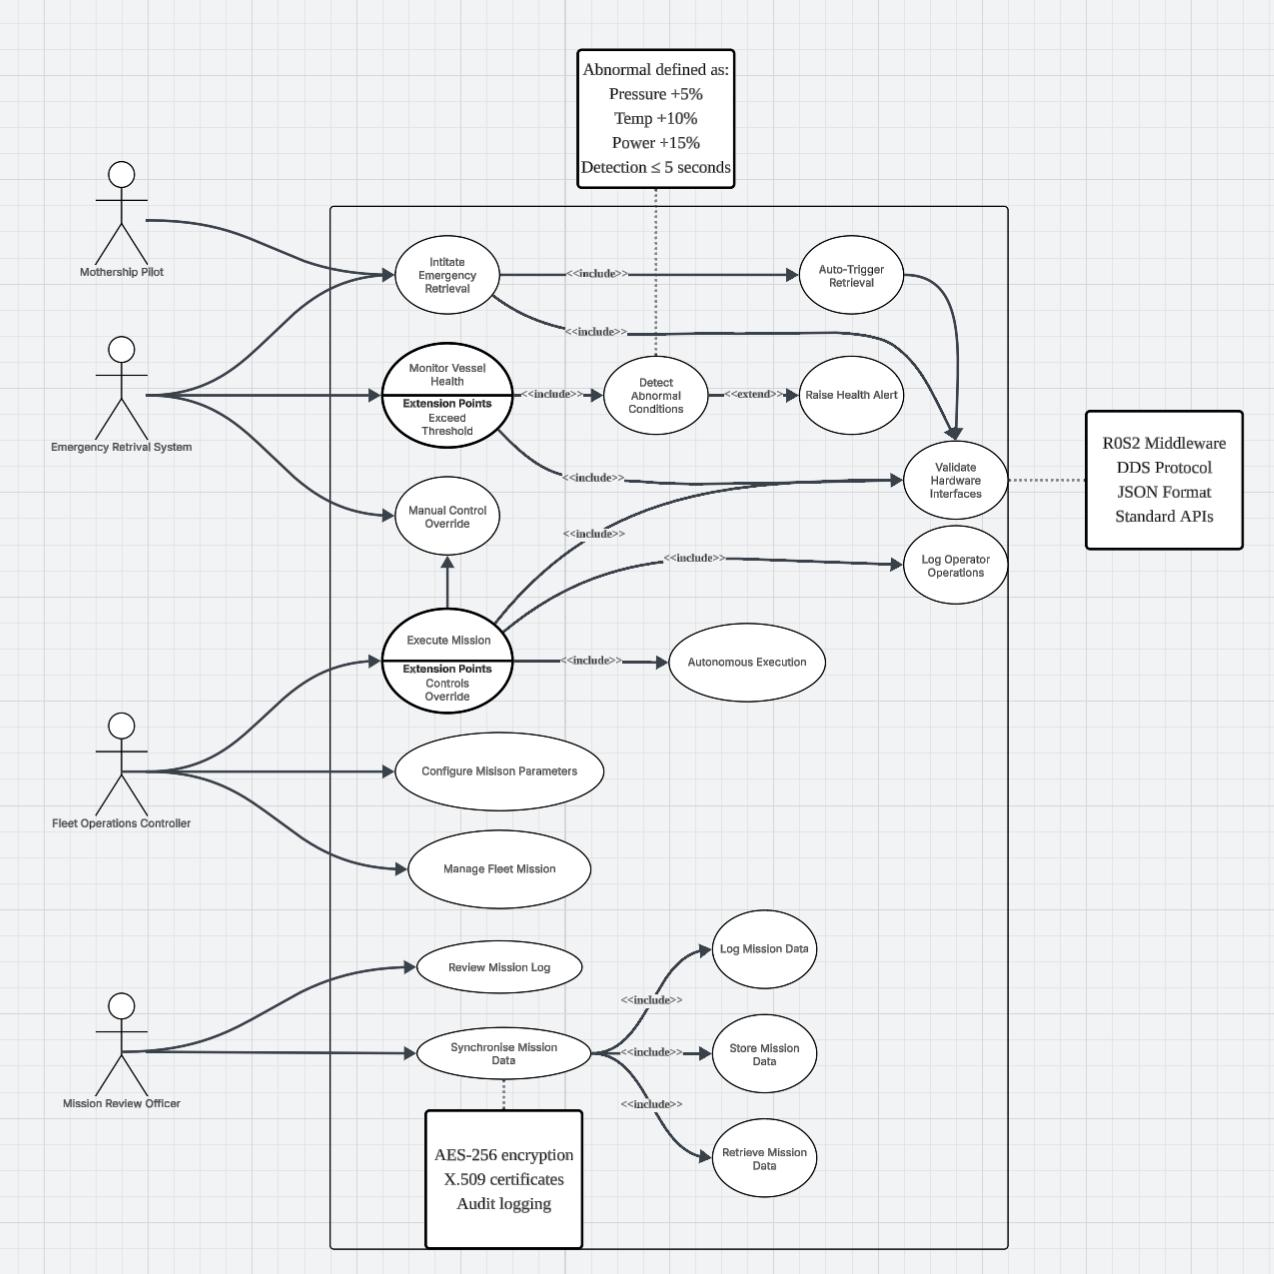
\includegraphics[width=0.85\textwidth]{../Models/UseCase Model.jpg}
\caption{Use Case Model: Representative operational interactions}
\label{fig:usecase-model}
\end{figure}

Additional Project Specification models (e.g., organization chart and roles/responsibilities) are adopted by reference from the Project Specification appendices to avoid divergence across artifacts.

% =====================
% 11. SIGN-OFF
% =====================
\section{Sign-off}
\label{sec:signoff}

\subsection{Vendor Authentication}
\begin{table}[H]
\centering
\small
\renewcommand{\arraystretch}{1.2}
\begin{tabular}{|p{0.28\textwidth}|p{0.22\textwidth}|p{0.4\textwidth}|}
\hline
\rowcolor{tableheader}
\textbf{Name} & \textbf{Employee ID} & \textbf{Signature} \\
\hline
Muhammad Ridwan Putra Jasni (Authenticator) & BDST-RE-BA-001 & \makebox[\linewidth][c]{
\includegraphics[height=1.2cm]{../Signatures/signature_ridwan.jpg}} \\
\hline
\end{tabular}
\caption{Vendor authenticator sign-off (signature provided)}
\end{table}

\subsection{Designated Approvers (No Signatures Required)}
\begin{table}[H]
\centering
\small
\renewcommand{\arraystretch}{1.2}
\begin{tabular}{|p{0.18\textwidth}|p{0.32\textwidth}|p{0.4\textwidth}|}
\hline
\rowcolor{tableheader}
\textbf{Organization} & \textbf{Role} & \textbf{Name (Designated)} \\
\hline
Customer (Triton Deepwater) & Project Leader / Requirements Approver & Sarah Whitman \\
\hline
Customer (Triton Deepwater) & Safety \& Compliance Approver & (TBD) \\
\hline
Vendor (Brigman) & Engineering Delivery Lead & (TBD) \\
\hline
Vendor (Brigman) & Verification \& Validation Lead & (TBD) \\
\hline
\end{tabular}
\caption{Designated approvers (placeholders where not yet nominated)}
\end{table}

\section*{Repository Information}
\addcontentsline{toc}{section}{Repository Information}
\begin{center}
\fbox{\begin{minipage}{0.9\textwidth}
\centering
\textbf{PROJECT REPOSITORY}\\[2pt]
\url{https://github.com/Spooky312/The-Abyss-Navigation-Suite-INF2113}\\[4pt]
\textit{SRS, models, and traceability artifacts maintained under version control}
\end{minipage}}
\end{center}

% =====================
% APPENDICES
% =====================
\appendix
\section{Glossary}
\begin{itemize}[leftmargin=*,nosep]
  \item \textbf{BCIC:} Breakdown, Clarify, Interpret, Categorize.
  \item \textbf{CRaM:} Correct, Relevant, and Measurable requirements organization principle.
  \item \textbf{iRTM:} Integrated Requirements Traceability Matrix.
  \item \textbf{Safe-state:} neutral buoyancy, minimal power, beacon active.
\end{itemize}

\section{To Be Determined (TBD) List}
\begin{itemize}[leftmargin=*,nosep]
  \item Customer nomination of Safety \& Compliance approver name.
  \item Final selection of database product/version for TECH-DB-001 (if different from PostgreSQL-equivalent).
  \item Final JSON schemas for INT-SENS-001 (to be published with the Interface/API guide).
\end{itemize}

\end{document}
